\section{Date: 2026-08-19}
\noindent \textbf{Series ID: BOPGG} 

\noindent This series is titled U.S. Government Grants Excluding Military (DISCONTINUED) and has a frequency of Quarterly. The units are Billions of Dollars and the seasonal adjustment is Seasonally Adjusted.The observation start date is 1960-01-01 and the observation end date is 2014-01-01.The popularity of this series is 1. \\ 

\noindent \textbf{Series ID: IPUBN212T051000000} 

\noindent This series is titled Sectoral Output Price Deflator for Mining: Mining (Except Oil and Gas) (NAICS 212) in the United States and has a frequency of Annual. The units are Percent Change from Year Ago and the seasonal adjustment is Not Seasonally Adjusted.The observation start date is 1988-01-01 and the observation end date is 2025-01-01.The popularity of this series is 1. \\ 

\subsection{Raw Regression}
\noindent Regresses the two series against each other directly. A significant result here can come just as easily from both series sharing a long-run trend as from any real relationship.

\begin{center}
\begin{tabular}{lclc}
\toprule
\textbf{Dep. Variable:}     & value\_fred\_IPUBN212T051000000 & \textbf{  R-squared:         } &     0.117   \\
\textbf{Model:}             &               OLS               & \textbf{  Adj. R-squared:    } &     0.082   \\
\textbf{Method:}            &          Least Squares          & \textbf{  F-statistic:       } &     3.328   \\
\textbf{Date:}              &         Wed, 19 Aug 2026        & \textbf{  Prob (F-statistic):} &   0.0801    \\
\textbf{Time:}              &             12:19:54            & \textbf{  Log-Likelihood:    } &   -85.697   \\
\textbf{No. Observations:}  &                  27             & \textbf{  AIC:               } &     175.4   \\
\textbf{Df Residuals:}      &                  25             & \textbf{  BIC:               } &     178.0   \\
\textbf{Df Model:}          &                   1             & \textbf{                     } &             \\
\textbf{Covariance Type:}   &            nonrobust            & \textbf{                     } &             \\
\bottomrule
\end{tabular}
\begin{tabular}{lcccccc}
                            & \textbf{coef} & \textbf{std err} & \textbf{t} & \textbf{P$> |$t$|$} & \textbf{[0.025} & \textbf{0.975]}  \\
\midrule
\textbf{const}              &       1.3198  &        1.512     &     0.873  &         0.391        &       -1.794    &        4.434     \\
\textbf{value\_fred\_BOPGG} &      -0.3525  &        0.193     &    -1.824  &         0.080        &       -0.750    &        0.045     \\
\bottomrule
\end{tabular}
\begin{tabular}{lclc}
\textbf{Omnibus:}       &  2.801 & \textbf{  Durbin-Watson:     } &    0.785  \\
\textbf{Prob(Omnibus):} &  0.246 & \textbf{  Jarque-Bera (JB):  } &    1.507  \\
\textbf{Skew:}          &  0.532 & \textbf{  Prob(JB):          } &    0.471  \\
\textbf{Kurtosis:}      &  3.454 & \textbf{  Cond. No.          } &     10.3  \\
\bottomrule
\end{tabular}
%\caption{OLS Regression Results}
\end{center}

Notes: \newline
 [1] Standard Errors assume that the covariance matrix of the errors is correctly specified.

\begin{figure}
\centering
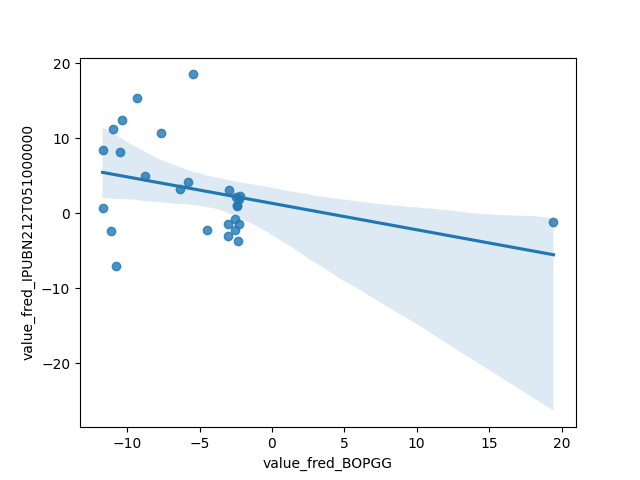
\includegraphics[scale = 0.9]{plots/plot_2026-08-19.png}
\caption{Raw Regression Plot for 2026-08-19}
\end{figure}
\newpage
\subsection{Detrended Regression}
\noindent Regresses the residuals of each series after removing its own linear time trend, so a shared trend can no longer drive the result on its own. A relationship that stays significant here is better evidence of a genuine link between the two series.

\begin{center}
\begin{tabular}{lclc}
\toprule
\textbf{Dep. Variable:}                & value\_fred\_IPUBN212T051000000\_detrended & \textbf{  R-squared:         } &     0.016   \\
\textbf{Model:}                        &                    OLS                     & \textbf{  Adj. R-squared:    } &    -0.024   \\
\textbf{Method:}                       &               Least Squares                & \textbf{  F-statistic:       } &    0.4017   \\
\textbf{Date:}                         &              Wed, 19 Aug 2026              & \textbf{  Prob (F-statistic):} &    0.532    \\
\textbf{Time:}                         &                  12:19:54                  & \textbf{  Log-Likelihood:    } &   -85.249   \\
\textbf{No. Observations:}             &                       27                   & \textbf{  AIC:               } &     174.5   \\
\textbf{Df Residuals:}                 &                       25                   & \textbf{  BIC:               } &     177.1   \\
\textbf{Df Model:}                     &                        1                   & \textbf{                     } &             \\
\textbf{Covariance Type:}              &                 nonrobust                  & \textbf{                     } &             \\
\bottomrule
\end{tabular}
\begin{tabular}{lcccccc}
                                       & \textbf{coef} & \textbf{std err} & \textbf{t} & \textbf{P$> |$t$|$} & \textbf{[0.025} & \textbf{0.975]}  \\
\midrule
\textbf{const}                         &   -1.801e-13  &        1.138     & -1.58e-13  &         1.000        &       -2.343    &        2.343     \\
\textbf{value\_fred\_BOPGG\_detrended} &      -0.1728  &        0.273     &    -0.634  &         0.532        &       -0.734    &        0.389     \\
\bottomrule
\end{tabular}
\begin{tabular}{lclc}
\textbf{Omnibus:}       &  2.027 & \textbf{  Durbin-Watson:     } &    0.686  \\
\textbf{Prob(Omnibus):} &  0.363 & \textbf{  Jarque-Bera (JB):  } &    0.803  \\
\textbf{Skew:}          &  0.236 & \textbf{  Prob(JB):          } &    0.669  \\
\textbf{Kurtosis:}      &  3.700 & \textbf{  Cond. No.          } &     4.17  \\
\bottomrule
\end{tabular}
%\caption{OLS Regression Results}
\end{center}

Notes: \newline
 [1] Standard Errors assume that the covariance matrix of the errors is correctly specified.

\begin{figure}
\centering
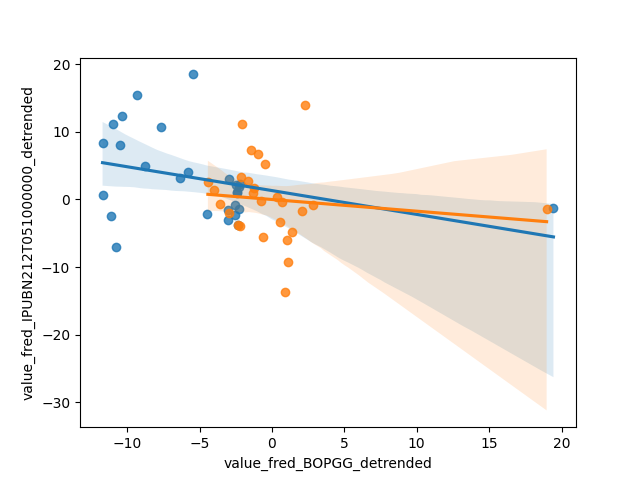
\includegraphics[scale = 0.9]{plots/plot_2026-08-19_detrended.png}
\caption{Detrended Regression Plot for 2026-08-19}
\end{figure}
\newpage
